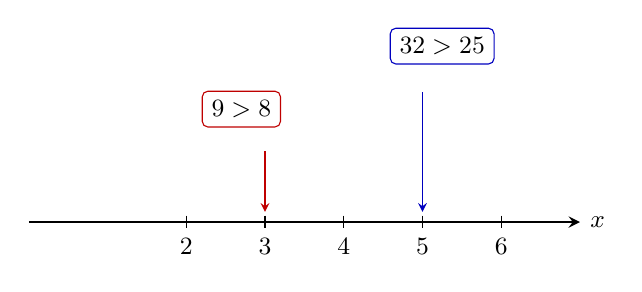
\begin{tikzpicture}[>=stealth,font=\small,x=1cm,y=1cm]
		\draw[->,thick] (0,0)--(7,0) node[right] {$x$};
		\foreach \x in {2,3,4,5,6} {\draw (\x,0.08)--(\x,-0.08) node[below]{\x};}
		\node[draw=red!75!black,rounded corners=2pt,above] at (2.7,1.2) {$9>8$};
		\node[draw=blue!75!black,rounded corners=2pt,above] at (5.25,2.0) {$32>25$};
		\draw[->,red!75!black] (3,0.9)--(3,0.13);
		\draw[->,blue!75!black] (5,1.65)--(5,0.13);
	\end{tikzpicture}
